\documentclass[10pt,aspectratio=169]{beamer}
\usefonttheme{professionalfonts}
\usepackage[utf8]{inputenc}
\usepackage{fontspec}
\usepackage{minted}
\usepackage{unicode-math}
\setsansfont{Roboto Light}
\setmonofont{DejaVu Sans Mono}
\usepackage{hyperref}
% \setsansfont{Fira Sans}
% \setmathfont[Scale=MatchLowercase]{Fira Math}
\setmathfont{STIX Two Math}
\setmathrm{STIX Two Math}
\setboldmathrm{STIX Two Math}
% \usepackage{animate}
\usepackage[absolute,overlay]{textpos}
\usepackage{multimedia}
% \setmathfont{Fira Math Regular}
\title{\Large \bfseries Introduction to Logistic Regression}
\subtitle{CHE 358 Mock Lecture}
\author{Tian Tian}
\date{22 June 2023}
    

\begin{document}
    
\frame{\titlepage}


\begin{frame}
\frametitle{Perspective of Lecture}
\begin{enumerate}
\item The classification problem
\item Logistic regression vs linear regression
\item Fitting a logistic regression
\item Case study: Li-ion battery failure
\item Beyond logistic regression: neural networks
\end{enumerate}
\end{frame}

\begin{frame}
  \frametitle{Categorical Response Variables}

  Many engineering problems
  have \textbf{categorical} response variables instead of
  \textbf{continuous} ones:

  \begin{itemize}
    \item Diagnostics: 	a patient \textbf{obese} or \textbf{not obese}
\item Decision:      	a valve to be turned \textbf{on} or \textbf{off}
\item Data discretization:  \textbf{pass} or \textbf{fail} a material strength test
\item Describing types: \textbf{cubic}, \textbf{hexagonal},
  \textbf{triclinic} Bravais lattices, etc.

\end{itemize}

\vspace{2em}

In contrast, response variables suitable for linear regression are:
\begin{itemize}
\item Continuous and quantitative
\item Ordering is meaningful
\item Distance is meaningful
\end{itemize}


\end{frame}

\begin{frame}
  \frametitle{The Classification Problem}

  Given:
  \begin{enumerate}
  \item Dataset: $D = \{(X_{1}, y_{1}), (X_{2},y_{2}), \cdots , (X_{n}, y_{n})\}$
  \item Categorical response variable $y$: $y_{i} \in C$, $C = \{C_{1}, C_{2}, \cdots, C_{k}\}$
    
\item Find optimal classifier function: $p(X; \theta)$ that predicts the category using parameter set $\theta$
  \end{enumerate}

  \vspace{2em}

  What a classification model will achieve:
    \begin{enumerate}
    \item Predict the categorical label
    \item Decision boundary for separation
    \item Probability of outcome
    \end{enumerate}
  
\end{frame}

\begin{frame}
  \frametitle{Solving Classification Problem by Regression}

  If the classifier function $p(X; \theta)$ corresponds to the
  \textbf{probability} of the outcome belonging to one class, the
  classification problem can be solved by regression.

  \vspace{2em}

  \begin{figure}[t]
    \vspace{-2em}
     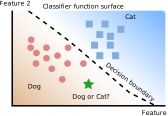
\includegraphics[width=0.6\textwidth]{images/classification_dog_cat.pdf}
    \end{figure}
  
  \end{frame}


\begin{frame}
  \frametitle{Thought Experiment: the Cheater’s Coin}
  
  You're a casino owner who wishes to create a biased coin. Can you
  come up with a model to fit your measurements?

  \vfill
  \begin{columns}[T]
    \begin{column}{0.20\textwidth}
      \begin{figure}[t]
        \includegraphics[width=\textwidth]{images/coin.pdf}
      \end{figure}
    \end{column}
    \begin{column}{0.75\textwidth}
      % \movie[loop]{}{scripts/animation.mp4}
      % \begin{figure}[t]
        % \animategraphics[width=\textwidth]{30}{scripts/animation-}{}{}
        % \includegraphics[width=\textwidth]{animation.gif}
      % \end{figure}
    \end{column}
  \end{columns}

\end{frame}

\begin{frame}
  \frametitle{First Try: Linear Regression for Classification Problems}
  \begin{columns}[T]
    \begin{column}{0.350\textwidth}
      Let's fit the dichotomous response variable $y_{i}$ by:
  \begin{equation*}
    p(x; \theta) = \beta_{0} + \beta_{1} x
  \end{equation*}

  Does linear regression makes sense?
  \begin{itemize}
  \item Range of predicted values?
  \item Distribution of residues?
  \item Are the predictions meaningful?
  \item Data extrapolation?
  \end{itemize}
\end{column}

\begin{column}{0.65\textwidth}
  \begin{figure}[t]
    \includegraphics[width=1.1\textwidth]{scripts/coin_linear_fit.pdf}
  \end{figure}
\end{column}
  \end{columns}
\end{frame}

\begin{frame}
  \frametitle{Why Not Linear Regression?}
  Linear regression is not suitable for classification problem:

  \begin{enumerate}
  \item \textbf{Invalid predicted values}

    Probability should be between $(0, 1)$
  
  \item \textbf{Assumption of linearity violated}

    Residuals are not independent of observation (not random)

  
  \item \textbf{Sensitive to data imbalance}

    If we have more "heavier-headed" coins sampled, the slope of linear regression will differ greatly.

    
  \item \textbf{Non-deterministic for multinomial classification}

    Should $C = \{\mathrm{Cat}, \mathrm{Dog}, \mathrm{Rabbit}\}$ be labeled as $\{0, 1, 2\}$ or $\{2, 1, 0\}$ or $\{0, 2, 6\}$?
    
  \end{enumerate}
\end{frame}

\begin{frame}
  \frametitle{Second Try: Non-Linear Regression}
  What are the properties of a non-linear $p(X; \theta)$?

  \vspace{1em}
  
  Recall: for binary response variables $(0, 1)$, $p$ is the probability of
  that the outcome is 1 (or vice-versa):
  \begin{equation*}
    p(X_{i}; \theta) = \mathrm{Prob}(y_{i}=1 | X=X_{i})
  \end{equation*}

  \vspace{1em}

  We could infer some properties of such probability distribution function:
  \begin{enumerate}
  \item \textbf{Range}:

    $p$ maps $X \in \mathbb{R}^{(m\times1)}$ to $y \in (0, 1)$.
    
  \item \textbf{Linearization}:

    A linear combination of $X$ can be separated to L.H.S via inversion function:

    \begin{equation*}
      p^{-1} = \mathrm{Inversion}(p) = X^{\mathrm{T}} \cdot \beta
    \end{equation*}

    where $\beta$ are the linear coefficients
  \item \textbf{Continuity}:

    To allow an analytical inversion form, $p$ should be continuous and monotonic.
    
  \end{enumerate}
  
\end{frame}

\begin{frame}
  \frametitle{How should $p$ look like?}

  A series of S-shaped (sigmoid) functions may meet our
  criteria. Let's check their plots in 1D.

  \vspace{-1em}
  \begin{figure}[t]
    \includegraphics[width=1.\textwidth]{scripts/sigmoid_funs.pdf}
  \end{figure}
  
\end{frame}

\begin{frame}
  \frametitle{The Logistic Function: Properties}
  
  In 1D form, the sigmoid function $p(z) = 1/(1 + \mathrm{exp}(-z))$ is called
  the \textbf{logistic function}. The process of fitting binary
  response variables is thus referred to as \textbf{logistic
    regression}.

    \begin{columns}[T]
      \begin{column}{0.5\textwidth}
        \begin{enumerate}
        \item Asymptotic behavior
          
          $\mathrm{lim}_{z\to\infty} p(z) = 1$ $\mathrm{lim}_{z\to-\infty} p(z) = 0$
          
        \item Symmetry

          $p(z) = 1 - p(1 -z)$
          
        \item Inflection point

          $p(0) = \frac{1}{2}$
          
        \item Inverse function

          $p^{-1} = \mathrm{log}(\frac{p}{1 - p})$

        \item 1st and 2nd Derivatives

          $p^{'}(z) = p(z)(1 - p(z))$

          $p^{''}(z) = p'(z)(1 - 2 p(z))$
        \end{enumerate}
      \end{column}

      \begin{column}{0.5\textwidth}

        \begin{figure}[t]
          \includegraphics[width=\textwidth]{scripts/logistic_fun_alone.pdf}
        \end{figure}
        
      \end{column}
      
    \end{columns}
  \end{frame}

  \begin{frame}
    \frametitle{Solving Logistic Regression: Ordinary Least Square?}
    
  \end{frame}

  \begin{frame}
    \frametitle{Fitting by Logistic Function: the Maximum Likelihood Estimation}

    A common approach to solve logistic regression is to maximize the
    \textbf{likelihood function} $L(\theta|D)$ of the logistic function by varying the
    parameter set $\theta$.

    The logistic regression problem is solved by find:

    \begin{equation*}
      \hat{\theta} = \mathrm{argmax}\ L(\theta|D)
    \end{equation*}
    
         \begin{figure}[t]
           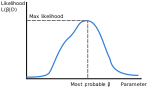
\includegraphics[width=0.5\textwidth]{images/likelihood.pdf}
         \end{figure}

    
  \end{frame}


  \begin{frame}
    \frametitle{The Likelihood of Logistic Function}

    The likelihood $L(\theta)$ of logistic functions follows the
    Bernoulli distribution:

        \begin{equation*}
          L(\theta|D) = \prod_{i=1}^{n} p_{i}^{y_{i}} (1 - p_{i})^{1-y_{i}}
        \end{equation*}

   Conventionally people also use the log-loss $l$:
        \begin{equation*}
          l(\theta|D) = -\mathrm{log}(L(\theta|D)) = \sum_{i=1}^{n} -y_{i} \mathrm{log}(p_{i}) -  (1 - y_{i}) \mathrm{log}(1 - p_{i})
        \end{equation*}
        
        where $p_{i} = \frac{1}{1 + \mathrm{exp}(- X_{i}^{{\mathrm{T}}} \cdot \beta)}$.
        $l(\theta|D)$ is the cost function of logistic regression.
        \\
        
        Now we just need to solve $\hat{\theta} = \mathrm{argmin}\ l(\theta|D)$.
        
      \end{frame}

      \begin{frame}
        \frametitle{Visualize the Cost Function}
        Let's take a look at the cost function if there is only 1 datum.
        
        \begin{columns}[T]
          \begin{column}{0.5\textwidth}
          \begin{equation*}
          y = 1
        \end{equation*}
                  \vspace{-4em}
            \begin{figure}[t]
              \includegraphics[width=0.75\textwidth]{scripts/loss_1.pdf}
            \end{figure}
          \end{column}

          \begin{column}{0.5\textwidth}
            \begin{equation*}
            y = 0
          \end{equation*}
          \vspace{-4em}
            \begin{figure}[t]
              \includegraphics[width=0.75\textwidth]{scripts/loss_2.pdf}
            \end{figure}
          \end{column}
          
        \end{columns}
      \end{frame}

      \begin{frame}
        \frametitle{Numerical Optimization of the Cost Function (1)}
        Unlike the least square, logistic regression's likelihood
        function \textbf{does not} have a closed-form solution. The minimal
        value of $l(\theta)$ has to be solved numerically.

        For $\theta = [\beta_{0}, \beta_{1}, \cdots, \beta_{d}]$, we need to know the
        derivative of $l$ w.r.t $\beta_{i}$.

        We can rewrite the cost function as:

        \begin{equation*}
          l(\theta|D) = \sum_{i=1}^{n}  -\log (1 - p_{i}) - y_{i} X_{i}^{T}\cdot \mathbf{\beta}
        \end{equation*}

        Then the first partial derivative is
        \begin{align*}
          \frac{\partial l}{\partial \beta_{j}}
          &= -\sum_{i=1}^{n} -\frac{1}{1 + \exp(-X^{T}\cdot \beta)} X_{ij} + y_{i}X_{ij} \\
          &= \sum_{i=1}^{n} (p_{i} - y_{i})X_{ij}\\
          &= \nabla_{j} l(\theta | D)
        \end{align*}

        where $X_{ij}$ is the $j$-th component of $X_{i}$ (if $j=0$, $X_{ij} = 1$)
      \end{frame}

      \begin{frame}
        \frametitle{Numerical Optimization of the Cost Function (2)}
        With the derivatives known, the gradient descent
        algorithms can be used to minimize $l(\theta)$:

        For each parameter $\beta_{j}$, we pick the initial guess
        $\beta_{j}^{0}$, compute $p$, $l$ and
        $\partial l/\partial \beta_{j}$. We then iteratively update
        $\beta_{j}$ by the Newton's method between steps $s$ and $s+1$:

        \begin{equation*}
          \beta_{j}^{s+1} = \beta_{j}^{s} - \alpha_{s} \dfrac{l(\theta^{s}|D)}{\nabla_{j}l(\theta^{s} | D)}
        \end{equation*}

        where $\alpha_{s}$ is the \textit{learning rate} and $\theta^{s}$ is the parameter set at step $s$, respectively.

        We can further prove the cost function is a \textit{convex
          function}, meaning the gradient descent method is guaranteed
        to find the global minimal of $l(\theta | D)$.
        
      \end{frame}

      \begin{frame}
        \frametitle{Visualize the Gradient Descent}

        In practice, many other methods like the
        Broyden–Fletcher–Goldfarb–Shanno (BFGS) algorithm have better
        performance than the Newton's method.
      \end{frame}

      \begin{frame}
        \frametitle{Caveat: Regularization}
        Consider a ``perfectly-separable'' binary
        dataset. Unconstrained logistic regression may result in large
        $\beta_{j}$ coefficients, leading to \textbf{overfitting}. How
        can we avoid this?

        \begin{figure}[t]
          \includegraphics[width=0.90\textwidth]{scripts/perfect_sep.pdf}
        \end{figure}
        
      \end{frame}

      \begin{frame}
        \frametitle{Regularization (1)}

        We can add additional penalty terms $P(\theta)$ to our cost
        function to penalize large coefficients (weights). Two
        commonly used regularization methods in statistics and machine
        learning are:

        \begin{itemize}
        \item L1 (lasso) regularization
          \begin{equation*}
            P(\theta) = \sum_{j=0}^{d} |\beta_{j}| 
          \end{equation*}

          
        \item L2 (ridge) regularization
          \begin{equation*}
            P(\theta) = \sum_{j=0}^{d} \beta_{j}^{2}
          \end{equation*}
        \end{itemize}

        The full cost function $C(\theta)$ for logistic regression is then:
        \begin{equation*}
          C(\theta) = l(\theta) + \lambda P(\theta)
        \end{equation*}
        where $\lambda$ is the strength of regularization penalty. The
        choice of L1 or L2 depends on the problem.
      \end{frame}

      \begin{frame}
        \frametitle{Regularization (2)}
        Let's see how regularization helps in the previous case
        (perfectly-separable dataset):

        \begin{figure}[t]
          \includegraphics[width=0.95\textwidth]{scripts/perfect_sep_reg.pdf}
        \end{figure}
      \end{frame}

      \begin{frame}
        \frametitle{Logistic Regression Demo: Cheater’s Coin}
        \begin{columns}[T]
          \begin{column}{0.5\textwidth}
            Logistic regression using Python's scikit-learn library:
            
            \inputminted[fontsize=\scriptsize]{python}{sample_lr_coin.py}
          \end{column}

          \begin{column}{0.5\textwidth}
            \begin{figure}[t]
              \includegraphics[width=\textwidth]{scripts/coin_fit_lr.pdf}
            \end{figure}
          \end{column}
        \end{columns}
      \end{frame}

      \begin{frame}
        \frametitle{How Do We Measure the Performance?}
        
      \end{frame}

      \begin{frame}
        \frametitle{Real-World Example: Li-ion Battery Failure (1)}

        Can you predict if a lithium-ion battery in EV will fail from measurements\let\thefootnote\relax\footnote{{\tiny Zhao et al. \textit{iScience} \textbf{25}, 104172}}?

        \begin{figure}[t]
          \includegraphics[width=0.9\linewidth]{images/battery_1.png}
        \end{figure}

      \end{frame}

      \begin{frame}
        \frametitle{Real-World Example: Li-ion Battery Failure (2)}
        Battery failure dataset. \let\thefootnote\relax\footnote{{\tiny Zhao et al. \textit{iScience} \textbf{25}, 104172}}.

        \begin{figure}[t]
          \includegraphics[width=1.0\linewidth]{images/battery_2.png}
        \end{figure}
      \end{frame}

      \begin{frame}
        \frametitle{Real-World Example: Li-ion Battery Failure (3)\let\thefootnote\relax\footnote{{\tiny See course material \url{https://github.com/alchem0x2A/uoa_che358_mock}}}}

        \begin{itemize}
        \item Step 1: Dataset split (train / test)

              Rule of thumb: 80/20 or 70/30 rule
          
        \item Step 2: Create a logistic regression model

              See our example in coin dataset
          
        \item Step 3: Hyper-parameter tuning

          Some hyper-parameters (e.g. regularization) may affect model performance beyond $\theta$
          
        \item Step 4: Model accuracy test

          Additional dataset or cross-validation
        \end{itemize}
        
        
      \end{frame}

      \begin{frame}
        \frametitle{Real-World Example: Li-ion Battery Failure (4)\let\thefootnote\relax\footnote{{\tiny See course material \url{https://github.com/alchem0x2A/uoa_che358_mock}}}}

        
        
        
      \end{frame}

      \begin{frame}
        \frametitle{Advanced Topic: Logistic Regression to Neural Network (1)}
        In machine learning, the logistic regression can be viewed as
        a single perceptron (neuron).

        
      \end{frame}

      \begin{frame}
        \frametitle{Advanced Topic: Logistic Regression to Neural Network (2)}
        We can extend the single ``logistic perceptron'' to a complex ``neural network''.
        
      \end{frame}

      \begin{frame}
        \frametitle{Advanced Topic: Logistic Regression to Neural Network (3)}
        
      \end{frame}

      \begin{frame}
        \frametitle{Advanced Topic: Logistic Regression to Neural Network (4)}
        
      \end{frame}

      \begin{frame}
        \frametitle{Recap: Linear Regression vs Logistic Regression}
        
      \end{frame}

      \begin{frame}
        \frametitle{Open Questions}

        \begin{enumerate}
        \item Could you think of a way to extend binary logistic regression for multinomial classification problems?

          
        \item Could you prove that the logistic function's log-loss is a convex function?

          
        \item What if we use other sigmoid functions (e.g. scaled $\tanh$) for ``logistic'' regression? Could you compare the model robustness and computational expenses?
        
        \end{enumerate}
        
      \end{frame}

      \begin{frame}[c]
        \frametitle{}
        \centering
        \vspace{3em}
        {\Huge \bfseries Questions?}
      \end{frame}
      
    
    
\end{document}
